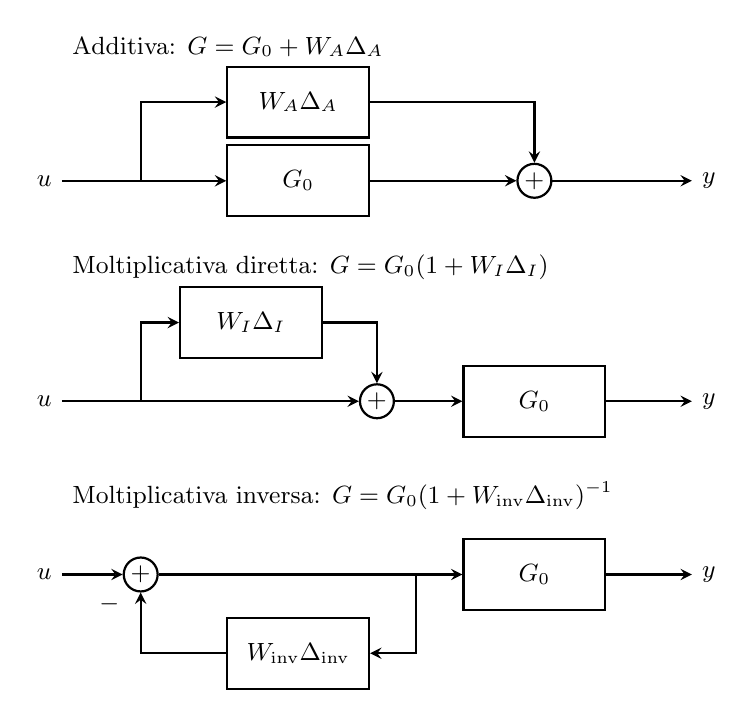
\begin{tikzpicture}[>=stealth,thick,every node/.style={font=\small},box/.style={draw,minimum width=18mm,minimum height=9mm},sum/.style={draw,circle,inner sep=1pt}]
\node[anchor=west] at (-1,1.7) {Additiva: $G=G_0+W_A\Delta_A$};
\node[box] (a) at (2,0) {$G_0$}; \node[sum] (s) at (5,0) {$+$};
\node[box] (d) at (2,1) {$W_A\Delta_A$};
\draw[->](-1,0)node[left]{$u$}--(a);\draw[->](a)--(s);\draw[->](s)--(7,0)node[right]{$y$};
\draw[->](0,0)|-(d);\draw[->](d)-|(s);
\node[anchor=west] at (-1,-1.1) {Moltiplicativa diretta: $G=G_0(1+W_I\Delta_I)$};
\node[sum] (t) at (3,-2.8) {$+$};\node[box] (b) at (5,-2.8) {$G_0$};
\node[box] (e) at (1.4,-1.8) {$W_I\Delta_I$};
\draw[->](-1,-2.8)node[left]{$u$}--(t);\draw[->](t)--(b);\draw[->](b)--(7,-2.8)node[right]{$y$};
\draw[->](0,-2.8)|-(e);\draw[->](e)-|(t);
\node[anchor=west] at (-1,-4) {Moltiplicativa inversa: $G=G_0(1+W_{\rm inv}\Delta_{\rm inv})^{-1}$};
\node[sum] (v) at (0,-5) {$+$};\node[box] (c) at (5,-5) {$G_0$};
\node[box] (f) at (2,-6) {$W_{\rm inv}\Delta_{\rm inv}$};
\draw[->](-1,-5)node[left]{$u$}--(v);\draw[->](v)--(c);\draw[->](c)--(7,-5)node[right]{$y$};
\draw[->](3.5,-5)|-(f);\draw[->](f)-|(v)node[below left=4pt]{$-$};
\end{tikzpicture}
